
%% Based on a TeXnicCenter-Template by Tino Weinkauf.
%%%%%%%%%%%%%%%%%%%%%%%%%%%%%%%%%%%%%%%%%%%%%%%%%%%%%%%%%%%%%

%%%%%%%%%%%%%%%%%%%%%%%%%%%%%%%%%%%%%%%%%%%%%%%%%%%%%%%%%%%%%
%% HEADER
%%%%%%%%%%%%%%%%%%%%%%%%%%%%%%%%%%%%%%%%%%%%%%%%%%%%%%%%%%%%%
\documentclass[a4paper,twoside,10pt]{report}
% Alternative Options:
%	Paper Size: a4paper / a5paper / b5paper / letterpaper / legalpaper / executivepaper
% Duplex: oneside / twoside
% Base Font Size: 10pt / 11pt / 12pt


%% Language %%%%%%%%%%%%%%%%%%%%%%%%%%%%%%%%%%%%%%%%%%%%%%%%%
\usepackage[francais]{babel} %francais, polish, spanish, ...
\usepackage[T1]{fontenc}
\usepackage[utf8]{inputenc}
\usepackage{comment}
\usepackage[final]{pdfpages} 

\usepackage{lmodern} %Type1-font for non-english texts and characters


%% Packages for Graphics & Figures %%%%%%%%%%%%%%%%%%%%%%%%%%
\usepackage{graphicx} %%For loading graphic files
%\usepackage{subfig} %%Subfigures inside a figure
%\usepackage{pst-all} %%PSTricks - not useable with pdfLaTeX

%% Please note:
%% Images can be included using \includegraphics{Dateiname}
%% resp. using the dialog in the Insert menu.
%% 
%% The mode "LaTeX => PDF" allows the following formats:
%%   .jpg  .png  .pdf  .mps
%% 
%% The modes "LaTeX => DVI", "LaTeX => PS" und "LaTeX => PS => PDF"
%% allow the following formats:
%%   .eps  .ps  .bmp  .pict  .pntg


%% Math Packages %%%%%%%%%%%%%%%%%%%%%%%%%%%%%%%%%%%%%%%%%%%%
\usepackage{amsmath}
\usepackage{amsthm}
\usepackage{amsfonts}


%% Line Spacing %%%%%%%%%%%%%%%%%%%%%%%%%%%%%%%%%%%%%%%%%%%%%
%\usepackage{setspace}
%\singlespacing        %% 1-spacing (default)
%\onehalfspacing       %% 1,5-spacing
%\doublespacing        %% 2-spacing


%% Other Packages %%%%%%%%%%%%%%%%%%%%%%%%%%%%%%%%%%%%%%%%%%%
%\usepackage{a4wide} %%Smaller margins = more text per page.
\usepackage{fancyhdr} %%Fancy headings
%\usepackage{longtable} %%For tables, that exceed one page


%%%%%%%%%%%%%%%%%%%%%%%%%%%%%%%%%%%%%%%%%%%%%%%%%%%%%%%%%%%%%
%% Remarks
%%%%%%%%%%%%%%%%%%%%%%%%%%%%%%%%%%%%%%%%%%%%%%%%%%%%%%%%%%%%%
%
% TODO:
% 1. Edit the used packages and their options (see above).
% 2. If you want, add a BibTeX-File to the project
%    (e.g., 'literature.bib').
% 3. Happy TeXing!
%
%%%%%%%%%%%%%%%%%%%%%%%%%%%%%%%%%%%%%%%%%%%%%%%%%%%%%%%%%%%%%

%%%%%%%%%%%%%%%%%%%%%%%%%%%%%%%%%%%%%%%%%%%%%%%%%%%%%%%%%%%%%
%% Options / Modifications
%%%%%%%%%%%%%%%%%%%%%%%%%%%%%%%%%%%%%%%%%%%%%%%%%%%%%%%%%%%%%

%\input{options} %You need a file 'options.tex' for this
%% ==> TeXnicCenter supplies some possible option files
%% ==> with its templates (File | New from Template...).



%%%%%%%%%%%%%%%%%%%%%%%%%%%%%%%%%%%%%%%%%%%%%%%%%%%%%%%%%%%%%
%% DOCUMENT
%%%%%%%%%%%%%%%%%%%%%%%%%%%%%%%%%%%%%%%%%%%%%%%%%%%%%%%%%%%%%
\begin{document}

\pagestyle{empty} %No headings for the first pages.


%% Title Page %%%%%%%%%%%%%%%%%%%%%%%%%%%%%%%%%%%%%%%%%%%%%%%
%% ==> Write your text here or include other files.

%% The simple version:
\title{Projet de Programmation}
\author{Alexandre Kervadec, Guillaume Verdugo, Jeremy Arrestier, Thibaut Fabre}
%\date{} %%If commented, the current date is used.
\maketitle

%% The nice version:
%\input{titlepage} %%You need a file 'titlepage.tex' for this.
%% ==> TeXnicCenter supplies a possible titlepage file
%% ==> with its templates (File | New from Template...).


%% Inhaltsverzeichnis %%%%%%%%%%%%%%%%%%%%%%%%%%%%%%%%%%%%%%%
\tableofcontents %Table of contents
\cleardoublepage %The first chapter should start on an odd page.

\pagestyle{plain} %Now display headings: headings / fancy / ...



%% Chapters %%%%%%%%%%%%%%%%%%%%%%%%%%%%%%%%%%%%%%%%%%%%%%%%%
%% ==> Write your text here or include other files.

%\input{intro} %You need a file 'intro.tex' for this.


%%%%%%%%%%%%%%%%%%%%%%%%%%%%%%%%%%%%%%%%%%%%%%%%%%%%%%%%%%%%%
%% ==> Eléments bibliographiques et présentation du projet:

\chapter{Présentation du projet}\label{resume_projet}

\section{Résumé}

Le projet qui nous est proposé, porte sur la relation entre prosodie et expression des sentiments. Notre but est de réaliser une interface graphique permettant de réaliser des tests prosodiques sur des cobayes.
Ces sujets auront à faire un choix, d’une vidéo parmi plusieurs, à fusionner avec une bande son parmi une autre liste.
Ce mixe de vidéo/son devra donner une réponse à une question du genre : “Réaliser une vidéo qui exprime l’excitation.”

\section{Approche logicielle du projet}

  \begin{figure}[h]
  \begin{center}
   \fbox{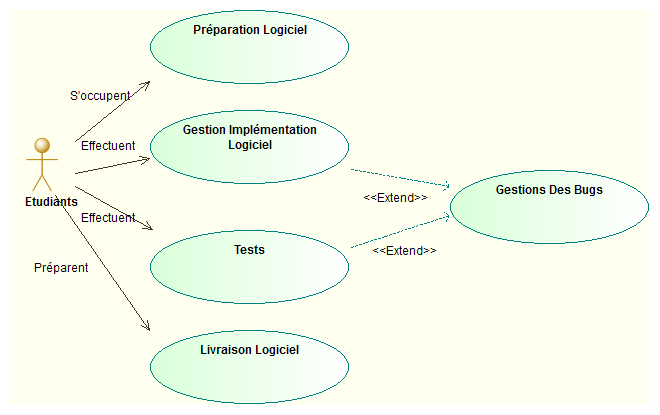
\includegraphics[width=\textwidth]{logiciel.png}}
   \caption{Diagramme de cas d'utilisation - Approche logicielle}
   \label{diaglog} 
  \end{center}
  \end{figure}
  
  Ce diagramme de cas d'utilisation (\textsc{Figure} \ref{diaglog}) présente l'approche génie logiciel du projet. Plus exactement les différentes étapes de développement de l'application.
  
\section{Approche du projet avec les différents acteurs}

  \begin{figure}[h]
  \begin{center}
   \fbox{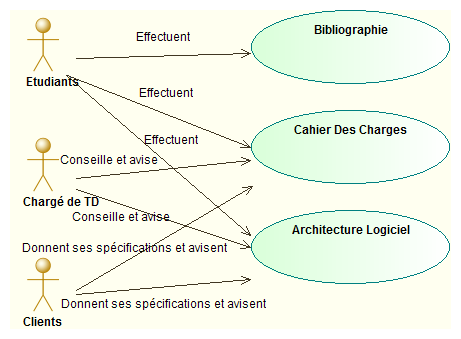
\includegraphics[width=\textwidth]{preparation.png}}
   \caption{Diagramme de cas d'utilisation - Approche Préparation projet}
   \label{diagact} 
  \end{center}
  \end{figure}
  
  Ce digramme de cas d'utilisation (\textsc{Figure} \ref{diagact}) expose les intéractions entre les différents acteurs du projet.
  
\section{Fonctionnement de l'application}
  
  \begin{figure}[h]
  \begin{center}
   \fbox{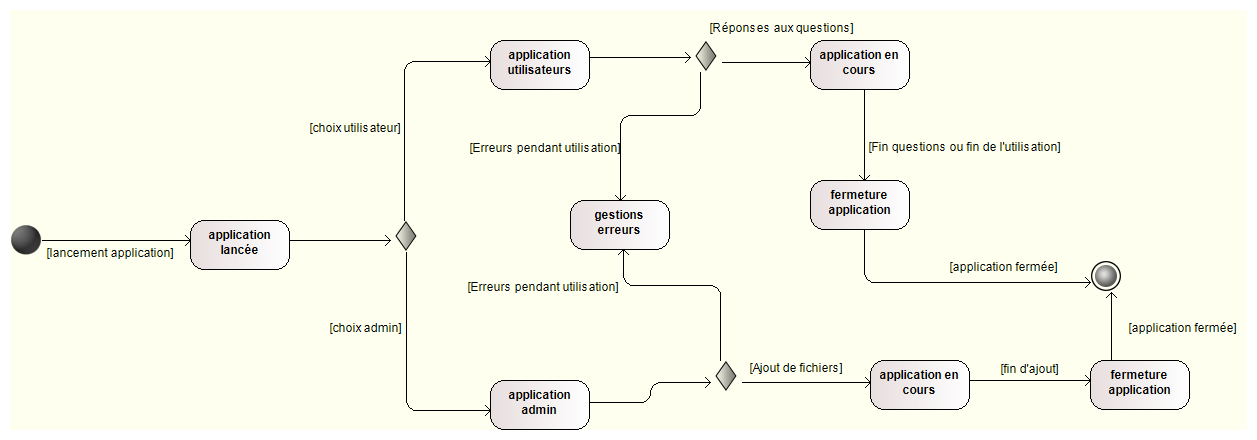
\includegraphics[width=20cm,angle=90]{etattrans.png}}
   \caption{Diagramme d'états - Fonctionnement de l'application}
   \label{etattrans}
  \end{center}
  \end{figure}
  
  La \textsc{Figure} \ref{etattrans} décrit le fonctionnement de l'application, \textit{i.e.} les différents états dans lesquels il est possible de se trouver durant l'utilisation de l'application.
  
  \begin{figure}[h]
  \begin{center}
   \fbox{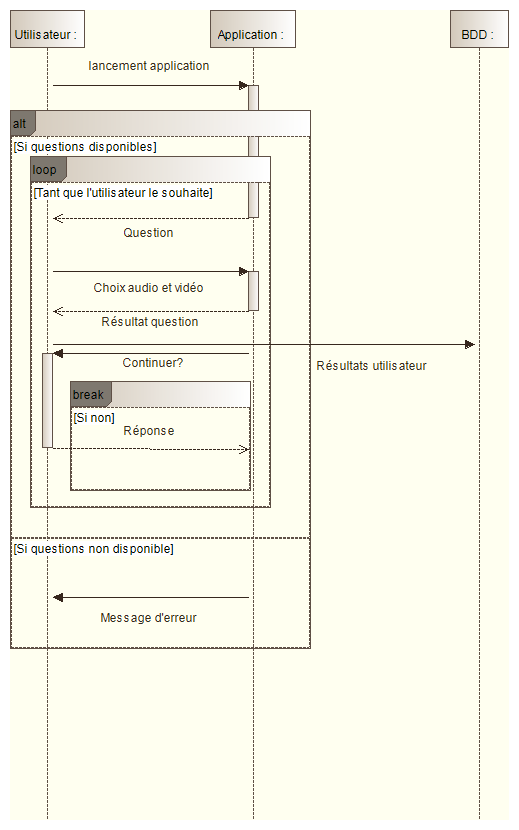
\includegraphics[width=10cm]{sequence.png}}
   \caption{Diagramme de séquences - Fonctionnement de l’application utilisateur mode Questions/Réponses}
   \label{sequence} 
  \end{center}
  \end{figure}
  
  La \textsc{Figure} \ref{sequence} est en rapport avec le diagramme précédent (\textsc{Figure} \ref{etattrans}). Il décrit les relations entre les différents états de transition.
  

\chapter{Analyse des besoins}\label{besoins}

\section{Classement par priorité des besoins}\label{priorite}

Les besoins sont classés par priorité dans leur ordre d'apparition. De plus, chaque besoin se voit attribué un niveau de priorité comme suit :

\begin{itemize}
  \item[-] Priorité critique
  \item[-] Priorité moyenne
  \item[-] Priorité basse
  \item[-] Facultatif
\end{itemize}


\section{Besoins fonctionnels}\label{besoins_fonctionnels}

\subsection{Utiliser l’application sur les systèmes d’exploitation principaux et récents}\label{systems}

\subsubsection{Description}
Etant donné que notre client sera amené à transporter l’application, il faut que celle-ci puisse fonctionner sur différents environnements à savoir \textit{Microsoft Windows 7}, \textit{Ubuntu 12.04}, \textit{Debian 6.0}, \textit{MAC OS X 10.9} et les versions plus récentes de ces systèmes d’exploitation.
L’application est susceptible de fonctionner sur d’autres systèmes d’exploitation (par compatibilité de noyau) sans toutefois de garantie de ce fonctionnement. 
\subsubsection{Faisabilité}

Cette condition sera remplie en utilisant une application web, supportée par tous les environnements possédant un navigateur web. Or cette qualité est remplie nativement par tous les systèmes d’exploitation cités précédemment.

\subsubsection{Contingence}

Le risque principal est que le client travaille sur une machine ne possédant pas de navigateur web. Pour pallier à cela, un navigateur web portable, comme par exemple \textit{Mozilla Firefox Portable Edition}, sera installé sur le périphérique utilisé.

\subsubsection{Test}

Lancer l'application dans chacun des systèmes d’exploitation cités précédemment.

\subsubsection{Priorité : \textit{Critique}}

\subsection{Rendre l’application nomade}\label{nomadite}

\subsubsection{Description}
Pour effectuer ses études, notre client ne souhaite pas transporter sa machine sur les lieux où elles se déroulent. Pour cela, il faut donc avoir une application transportable sur un périphérique externe de type clef USB.

\subsubsection{Faisabilité}

Pour remplir cette condition, tous les composants de l’application seront stockés sur une clef USB ou un disque dur externe afin que le client puisse l'utiliser sur n’importe quel ordinateur.


\subsubsection{Contingence}

Le risque serait que le formatage de la partition de la clef USB ne soit pas pris en compte par le système d’exploitation de la machine (par exemple le formatage \textit{NTFS} de \textit{Windows} n’est pas reconnu par le système \textit{Mac OS}, le formatage \textit{EXT4} du système \textit{Ubuntu} n’est pas reconnu par les systèmes d’exploitation \textit{Windows}). Pour éviter cela, la clef devra être formatée en \textit{FAT32} qui est un formatage de partition reconnu par les systèmes d’exploitation cités dans la section \ref{systems}.

\subsubsection{Test}

Faire fonctionner l’application à partir d’une clef USB (ou disque dur externe selon le support qui sera choisi).

\subsubsection{Priorité : \textit{Critique}}

\subsection{Ajouter du contenu multimédia et des questions}

\subsubsection{Description}
Le client doit pouvoir enregistrer dans la base de données, de nouvelles vidéos et de nouveaux sons afin d’augmenter l’efficience de ses tests. De plus, pour améliorer ses recherches, notre client pourra ajouter des questions avec leurs correspondances audios et vidéos.

\subsubsection{Faisabilité}

Pour faciliter cette gestion, nous utiliserons une base de données. Les données seront plus facilement accessibles lors de l’utilisation de l’application.

\subsubsection{Test}

Ajouter du contenu multimédia et une question puis lister tout le contenu de la base de données pour voir si l’ajout à été pris en compte.

\subsubsection{Priorité : \textit{Moyenne}}

\subsection{Exploiter différents formats de fichiers audio et vidéo}

\subsubsection{Description}


Le contenu multimédia de notre client étant composé de différents formats vidéos et audios, l’application doit pouvoir assurer une lecture optimale.

Effectivement, c’est un obstacle que l’on rencontre dès que l’on commence à programmer dans le domaine de la vidéo et de l’audio (des références étudiant certaines de ces contraintes : \cite{ghanbari1999video} et \cite{he2013introduction}).
Le fond du problème est l’utilisation de Codecs (vidéo et audio) pour lire les différents types de fichiers, qui sont encodés selon différentes normes.

Les formats que l’on doit pouvoir supporter sont les suivants :\\

%\begin{table} Fait planter le positionnement vertical du tableau.
\begin{center}
\begin{tabular}{c|c}
\textbf{Formats audio} & \textbf{Formats vidéo} \\
\\
\hline
\\
\textit{mpeg2} & \textit{mp4 (H.264)}\\
\textit{aac} & \textit{mov}\\
\textit{wav} & ~
\end{tabular}
\end{center}
%\end{table}
\vspace{0.6cm}

\subsubsection{Faisabilité}

Une solution que nous avons trouvé est le lecteur de médias \textit{VLC Media Player} \cite{solutions2006vlc}.

Ce lecteur va nous permettre d'utiliser les formats vidéo et audio présentés précédemment. De plus, c'est un logiciel accessible (gratuit et sous licence open-source).

De surcroit, il existe une version portable de \textit{VLC Media Player} permettant un transport optimal sur une clef USB ou un disque dur externe. Cette condition répond à notre besoin de transportabilité évoqué précédemment.

\subsubsection{Contingence}

Le risque d’utiliser ce genre de logiciel peut être l'impossibilité d'intégrer le lecteur dans une page web (solution choisie dans la section \ref{systems}), si l’application doit s’ouvrir dans un navigateur. Si cette solution n’est pas possible, on pourra ouvrir un lecteur indépendamment de la page web (en \textit{standalone}).

\subsubsection{Test}

Création d’un script qui ouvrira toutes les vidéos disponibles et vérifiera si une erreur est survenue.

\subsubsection{Priorité : \textit{Moyenne}}


%%%%%%%%%%%%%%%%%%%%%%%%%%%%%% Modifié le 04.02.2015 %%%%%%%%%%%%%%%%%%%%%%%%%%%%%%%%%%%%%%%%%%%%%%%

\subsection{Récupérer les questions et résultats des tests}

  \subsubsection{Description}

    L’application a pour but de répondre à une question donnée en fusionnant une vidéo et un audio.\\
    Ces combinaisons sont importantes pour notre client, nous devons donc les récupérer.

  \subsubsection{Faisabilité}

    La solution à ce besoin serait une base de données, stockant l’ensemble des questions, sons, vidéos et réponses/résultats.
    L’application devra aussi exporter les données sous forme d’un fichier \textit{txt}, fichier qu’exploitera le client.    

  \subsubsection{Test}

    Faire faire le test à un faux sujet, et vérifier les données exportées dans le fichier \textit{txt}.

  \subsubsection{Priorité : \textit{Moyenne}}


\subsection{Rassembler des informations sur les sujets}

  \subsubsection{Description}

    Afin de pouvoir exploiter les résultats des tests, le client veut récupérer des informations sur les sujets.
    Les informations que l’on doit récupérer sont les suivantes :\\
    \begin{itemize}
      \item[-]  nom
      \item[-]  prénom
      \item[-]  sexe
      \item[-]  date de naissance
      \item[-]  langue maternelle
      \item[-]  si la langue maternelle est différente de celle du test, nombre d’année d’études de cette langue
    \end{itemize}

  \subsubsection{Faisabilité}
    
    Pour répondre à ce besoin, il faut implémenter un formulaire au lancement de l’application.

  \subsubsection{Test}

    Faire essayer l’application à une personne tierce, puis, vérifier que toutes les informations sur la personne ont bien été récupérées.

  \subsubsection{Priorité : \textit{Faible}}



%%%%%%%%%%%%%%%%%%%%%%%%%%%% Fin de Modifié le 04.02.2015  %%%%%%%%%%%%%%%%%%%%%%%%%%%%%%%%%%%%%%%%%%


\section{Besoins non-fonctionnels}\label{besoins_non-fonctionnels}

\subsection{Permettre une maintenance du logiciel}

\subsubsection{Description}

L’application que nous allons livrer ne sera pas une finalité mais seulement une étape dans un projet beaucoup plus vaste. Ainsi, d’autres personnes devront probablement modifier cette application afin de répondre à de nouveaux besoins. Ces nouveaux développeurs devront disposer de tous les éléments nécessaires pour comprendre notre travail.                                                                                                                                                                                                                                                                                        
\subsubsection{Faisabilité}

Il est possible de répondre à ce besoin en documentant notre code. Il existe par exemple en \textit{Java}, la \textit{Javadoc}, qui est générable avec des commentaires spéciaux. Elle est exportable en \textit{PDF} et contient toutes les explications necessaires à la compréhension du code. Il existe aussi la \textit{PHPDoc} qui est l’équivalent pour le \textit{PHP}.

De plus, il faudra ajouter des commentaires quand une fonction sera trop complexe et que des indications intermédiaires seront nécessaires.

\subsubsection{Test}

Demander à un développeur externe au projet d’essayer de comprendre notre code.

\subsubsection{Priorité : \textit{moyenne}}

\begin{comment}
\subsection{Sécuriser les fonctionnalités d’ajout de contenu multimédia et de questions}

\subsubsection{Description}

La partie d’ajout doit être sécurisée. En effet, seul notre client possède le droit d’accroitre la quantité de contenu multimédia et de questions.\\
De plus, il faut que les vidéos et les sons insérés soient dans un format lisible par \textit{VLC Media Player}.

\subsubsection{Faisabilité}

Pour sécuriser la fonction d’ajout, un mot de passe unique, préalablement donné au client, sera demandé pour accéder à cette partie de l’application.\\
Lors de l’insertion de contenu multimédia, une vérification de format compatible à \textit{VLC Media Player} sera effectuée.

\subsubsection{Contingence}

Il se pourrait que le mot de passe soit oublié par le client ou volé par une personne malveillante.\\
Pour éviter le vol, le mot de passe sera encrypté sur la base de données.\\
Pour pallier l’oubli, un unique \textit{code PUK} lui sera fourni. Celui-ci sera demandé si le client souhaite modifier le mot de passe. Ce code sera aussi encrypté sur la base de données.

\subsubsection{Test}
Demander à une personne tierce, spécialisée en informatique, de tenter d’accéder à la partie sécurisée et de changer de mot de passe.\\
Tenter d’ajouter un fichier dans un format que ne prend pas en compte \textit{VLC Media Player}.

\subsubsection{Priorité : \textit{Moyenne}}
\end{comment}

\subsection{Bénéficier d’une ergonomie efficiente}

\subsubsection{Description}

L’application sera ergonomique pour permettre au sujet de se concentrer un maximum sur le test et pas sur le fonctionnement de ladite application. De plus, le sujet soumis au test sera possiblement novice en informatique, l’application devra ainsi être intuitive.

\subsubsection{Faisabilité}

Pour satisfaire ce besoin, nous devons mettre en place un graphisme épuré de tout accessoires détournant l’attention. De plus, nous utiliserons des couleurs de ton pastel pour éviter de fatiguer le regard de l’utilisateur.

Cette contrainte est satisfaisable en s’inspirant de nombreux designs qui ont déjà été développés et publiés sur le web. On s’appuiera notamment sur l’article \cite{lente2014scenariser} qui étudie la \textit{“collaboration entre Ergonomie, Design et Ingénierie”}.

\subsubsection{Test}

Se servir d'un novice en informatique pour tester l’application.

\subsubsection{Priorité : \textit{basse}}

\section{Prototype d'application}

  En annexe, un \textbf{\textit{prototype}} de l'application que nous allons développer est présenté. Le rendu final pourra différer de ce prototype.


\chapter{Organisation}

  \section{Gestion du temps}
  
  Nous avons établi un calendrier de projet qui présente le déroulement général du projet.
  
  \begin{figure}[h]
    \begin{center}
     \fbox{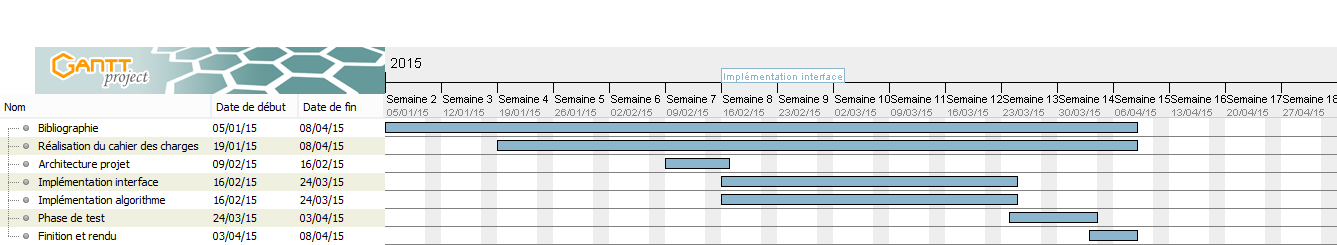
\includegraphics[width=18cm,angle=90]{gantt.png}}
     \caption{\label{gantt} Gantt - Calendrier du projet}
    \end{center}   
  \end{figure}


  
\chapter{Annexe}

  \section{Prototype}
  
 \begin{figure}[ht]
  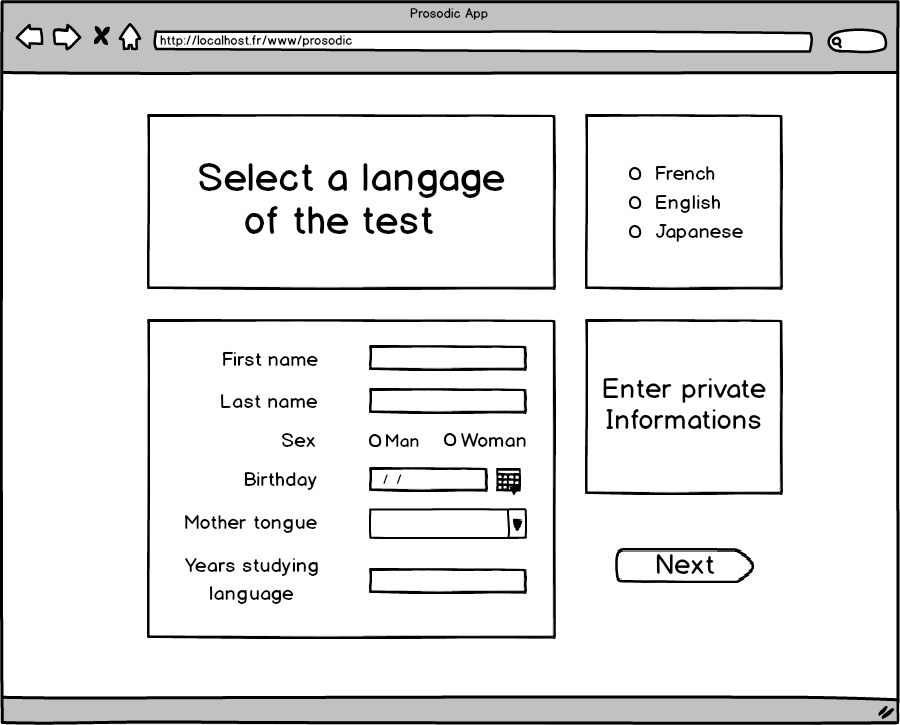
\includegraphics[width=\textwidth]{0.png}
 \end{figure}
 
 \begin{figure}[ht]
  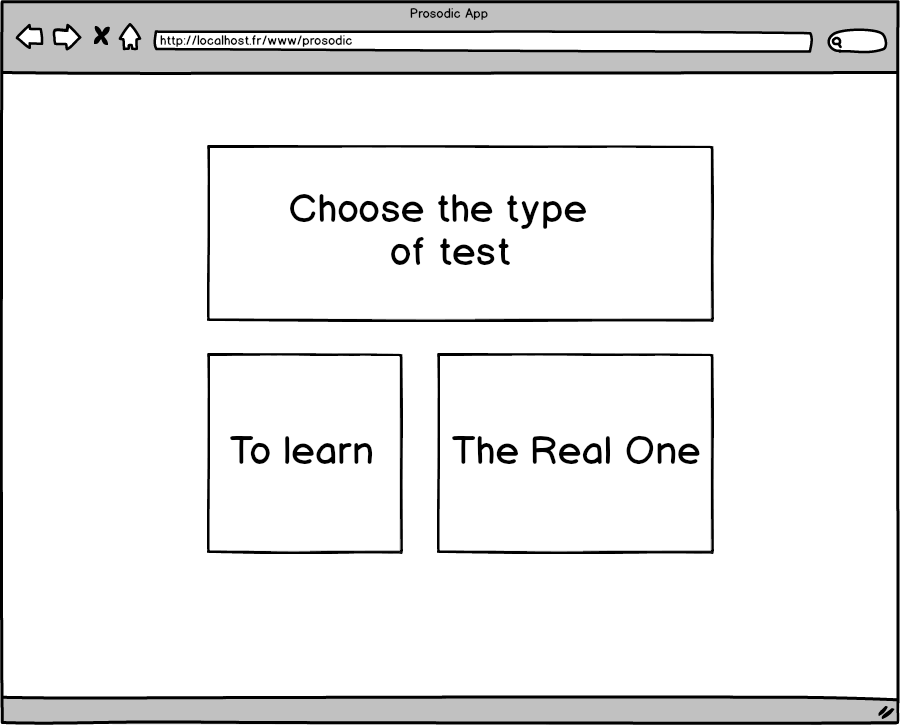
\includegraphics[width=\textwidth]{1.png}
 \end{figure}
 
 \begin{figure}[ht]
  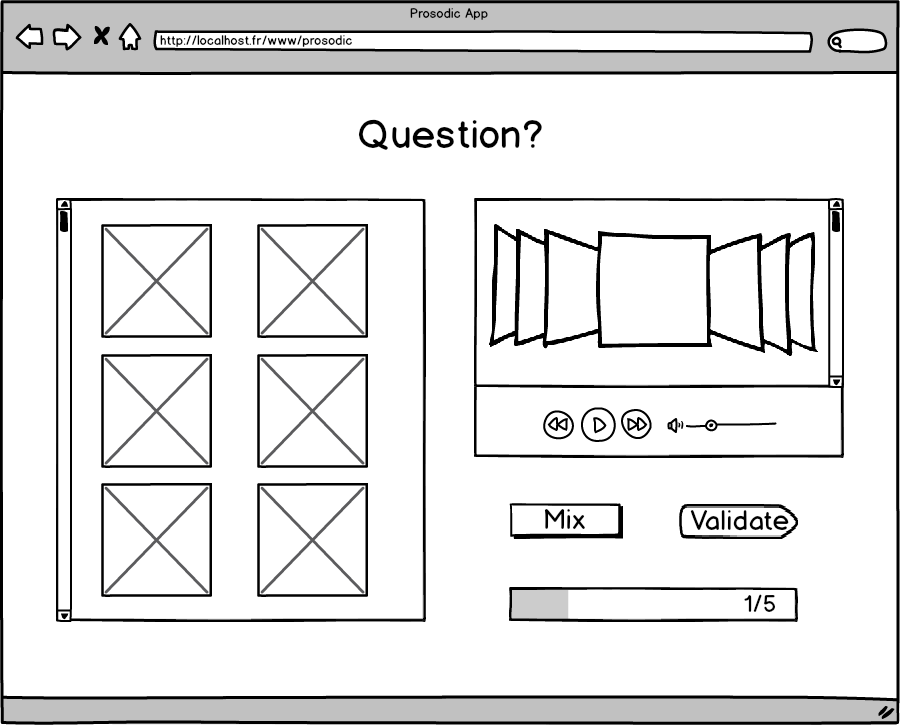
\includegraphics[width=\textwidth]{F-1.png}
 \end{figure}
 
 \begin{figure}[ht]
  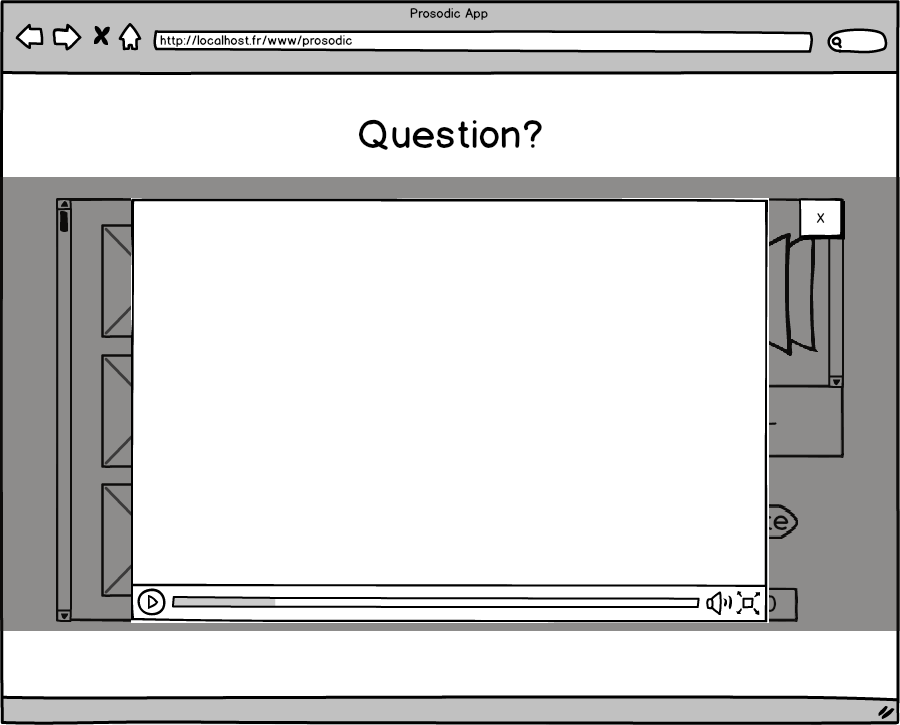
\includegraphics[width=\textwidth]{F-2.png}
 \end{figure}
 
 \begin{figure}[ht]
  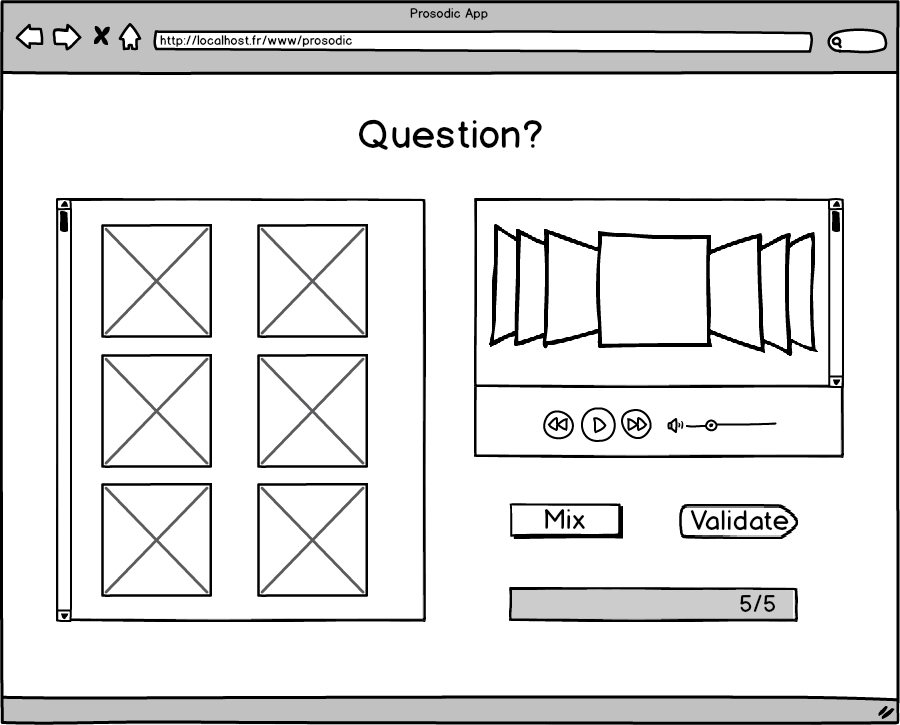
\includegraphics[width=\textwidth]{F-3.png}
 \end{figure}
 
 \begin{figure}[ht]
  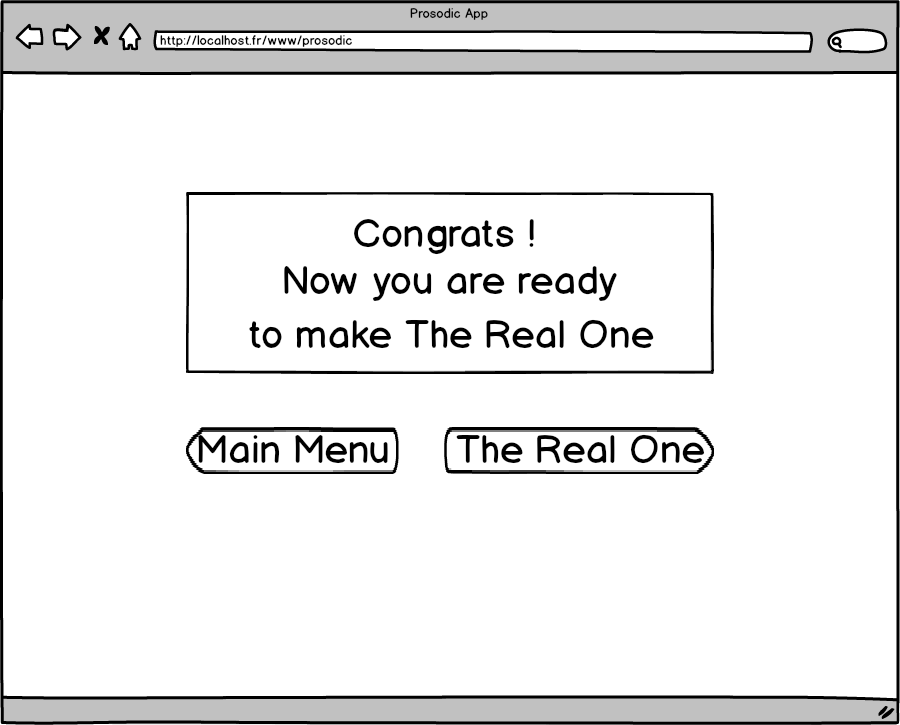
\includegraphics[width=\textwidth]{F-4.png}
 \end{figure}
 
 \begin{figure}[ht]
  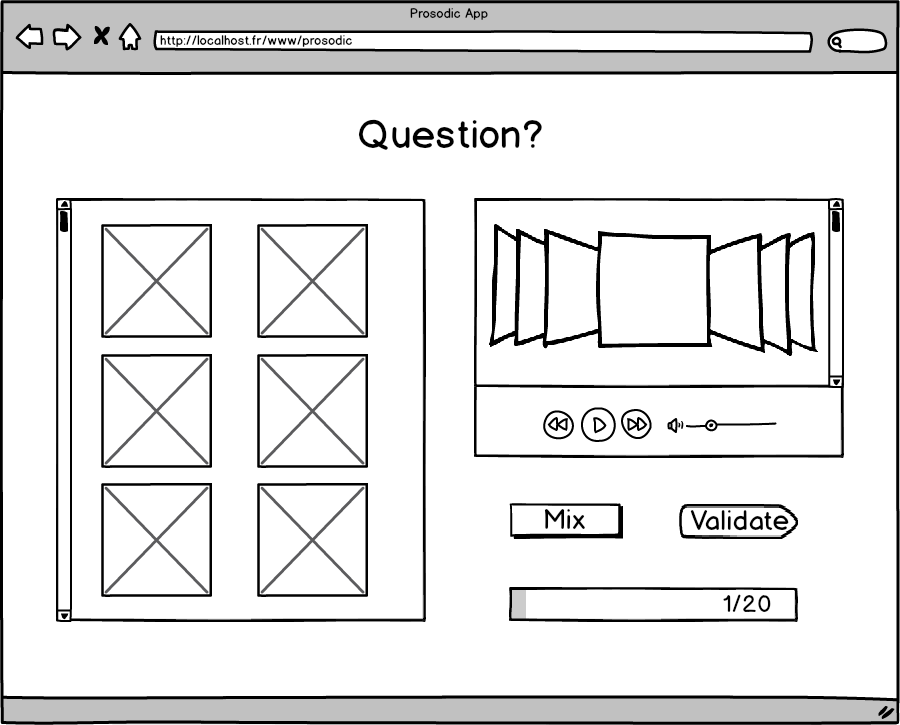
\includegraphics[width=\textwidth]{T-1.png}
 \end{figure}
 
 \begin{figure}[ht]
  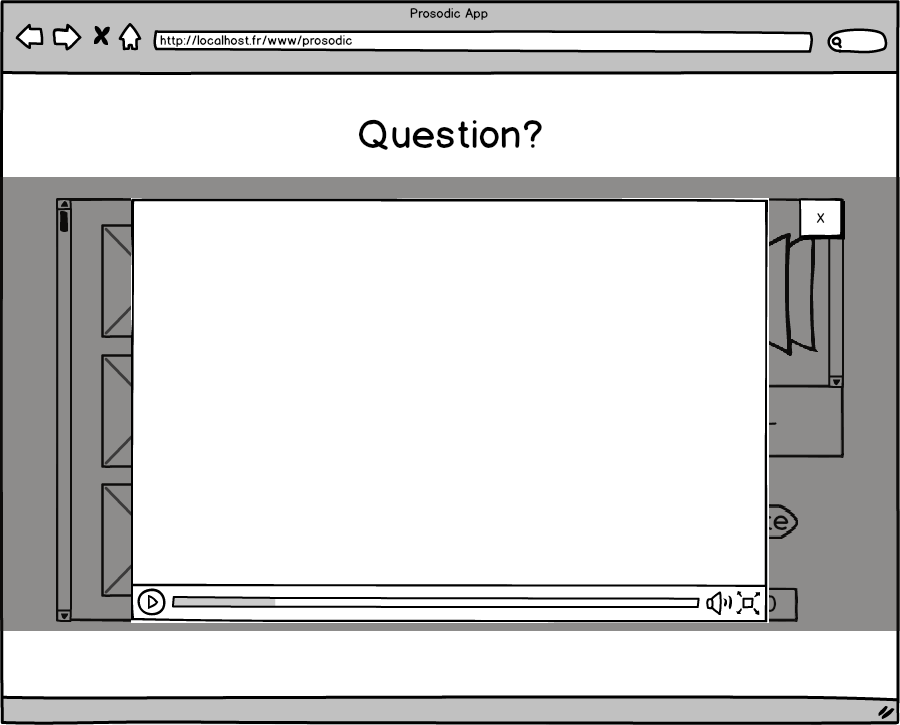
\includegraphics[width=\textwidth]{T-2.png}
 \end{figure}
 
 \begin{figure}[ht]
  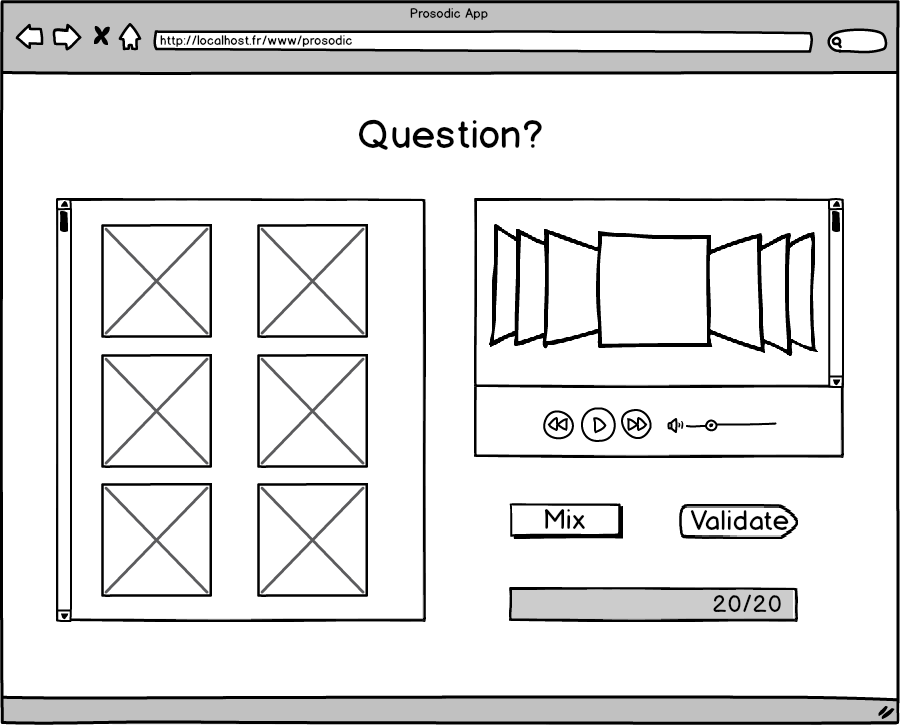
\includegraphics[width=\textwidth]{T-3.png}
 \end{figure}
 
 \begin{figure}[ht]
  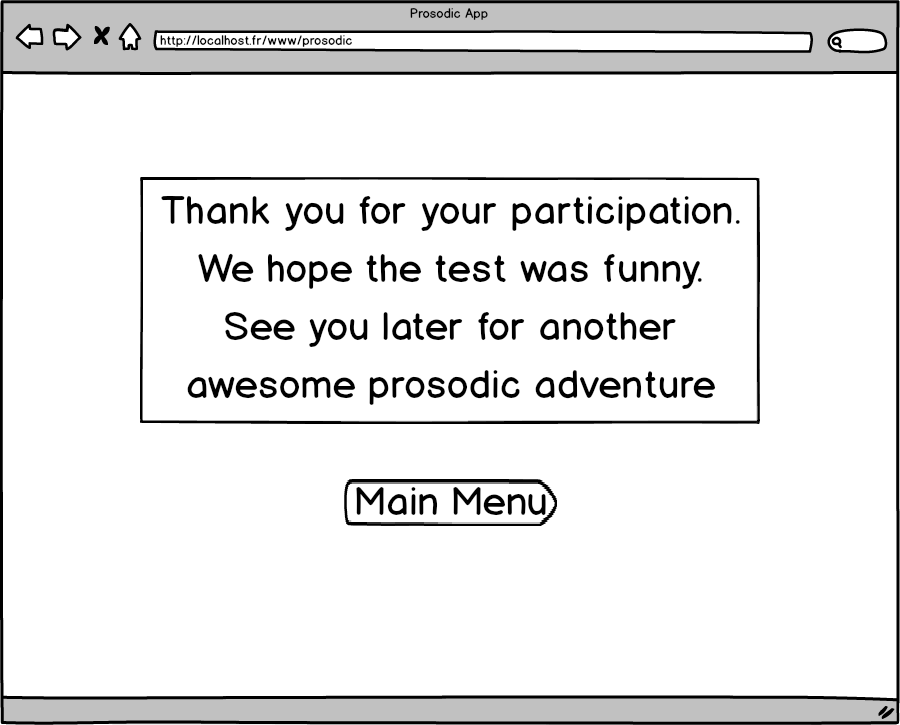
\includegraphics[width=\textwidth]{T-4.png}
 \end{figure}


%% <== 
%%%%%%%%%%%%%%%%%%%%%%%%%%%%%%%%%%%%%%%%%%%%%%%%%%%%%%%%%%%%%



%%%%%%%%%%%%%%%%%%%%%%%%%%%%%%%%%%%%%%%%%%%%%%%%%%%%%%%%%%%%%
%% BIBLIOGRAPHY AND OTHER LISTS
%%%%%%%%%%%%%%%%%%%%%%%%%%%%%%%%%%%%%%%%%%%%%%%%%%%%%%%%%%%%%
%% A small distance to the other stuff in the table of contents (toc)
\addtocontents{toc}{\protect\vspace*{\baselineskip}}

%% The Bibliography
%% ==> You need a file 'literature.bib' for this.
%% ==> You need to run BibTeX for this (Project | Properties... | Uses BibTeX)
\addcontentsline{toc}{chapter}{Bibliographie} %'Bibliography' into toc
\nocite{*} %Even non-cited BibTeX-Entries will be shown.
\bibliographystyle{alpha} %Style of Bibliography: plain / apalike / amsalpha / ...
\bibliography{literature} %You need a file 'literature.bib' for this.

%% The List of Figures
%\clearpage
%\addcontentsline{toc}{chapter}{List of Figures}
%\listoffigures

%% The List of Tables
%\clearpage
%\addcontentsline{toc}{chapter}{List of Tables}
%\listoftables


%%%%%%%%%%%%%%%%%%%%%%%%%%%%%%%%%%%%%%%%%%%%%%%%%%%%%%%%%%%%%
%% APPENDICES
%%%%%%%%%%%%%%%%%%%%%%%%%%%%%%%%%%%%%%%%%%%%%%%%%%%%%%%%%%%%%
\appendix
%% ==> Write your text here or include other files.

%\input{FileName} %You need a file 'FileName.tex' for this.


\end{document}

